\documentclass[aspectratio=169]{beamer}
\usefonttheme{serif}
\usepackage{xeCJK}
\usepackage{fontspec}
\usepackage{graphicx}
\usepackage{listings}
\usepackage{xcolor}
\usepackage{indentfirst}
\usepackage{tikz}
\usepackage{amssymb}
\usepackage{amsthm}
\usepackage{amsmath}
\usepackage{tabularx}
\usepackage{hyperref}
\usepackage{ulem}
\usepackage{version}
\usepackage{thmtools}
\usepackage{qtree}
\usepackage{algpseudocode}
\usepackage{mathtools}
\usepackage{multicol}
\usepackage{xcolor}

\AtBeginDocument{%
    \DeclareSymbolFont{pureletters}{T1}{\mathfamilydefault}{\mddefault}{it}%
    }

\XeTeXlinebreaklocale "zh"
\XeTeXlinebreakskip = 0pt plus 1pt

\setCJKmainfont{NotoSansTC-Medium.otf}
\setmainfont{JetBrainsMono-SemiBold.ttf}
\usetikzlibrary{arrows,decorations.markings,decorations.pathreplacing}
\newenvironment{Hint}{\noindent\textbf{Hint.}}{}

\tikzstyle {graph node} = [circle, draw, minimum width=1cm]
\tikzset{edge/.style = {decoration={markings,mark=at position 1 with %
            {\arrow[scale=2,>=stealth]{>}}},postaction={decorate}}}

\lstset{
    basicstyle=\ttfamily\normalsize,
    numberstyle=\normalsize,
    numbers=left,
    stepnumber=1,
    numbersep=3pt,
    commentstyle=\color{black!50},
    keywordstyle=\color{white!0!blue},
    stringstyle=\color{black!50!green},
    showspaces=false,
    showstringspaces=false,
    showtabs=false,
    tabsize=4,
    captionpos=b,
    breaklines=true,
    breakatwhitespace=false,
    escapeinside={\%*}{*)},
    morekeywords={*}
}

\AtBeginSection[]{
  \begin{frame}
  \vfill
  \centering
  \begin{beamercolorbox}[sep=8pt,center,shadow=true,rounded=true]{title}
    \usebeamerfont{title}\insertsectionhead\par%
  \end{beamercolorbox}
  \vfill
  \end{frame}
}

\title{圖論 I}
\author{Koying}
\date{2022-07-08}

\usetheme{Madrid}
\usecolortheme{default}
\setbeamertemplate{itemize items}[square]
\setbeamertemplate{enumerate items}[default]
\setbeamertemplate{blocks}[default]
\lstdefinestyle{myStyle}{
    belowcaptionskip=1\baselineskip,
    breaklines=true,
    frame=none,
    numbers=none, 
    basicstyle=\footnotesize\ttfamily,
    keywordstyle=\bfseries\color{green!40!black},
    commentstyle=\itshape\color{purple!40!black},
    identifierstyle=\color{blue},
    backgroundcolor=\color{gray!10!white},
}

\begin{document}

    \begin{frame}
        \titlepage
    \end{frame}

    \begin{frame}{目錄}
        \begin{itemize}
            \item 前言
            \item 圖的名詞
            \item 圖的儲存
            \item 圖的遍歷
            \item 二分圖
            \item 拓撲排序
            \item DAG 上的 DP
        \end{itemize}
    \end{frame}

    \section{前言}

    \begin{frame}{前言}
        \begin{itemize}
            \item 相信大家都或多或少聽過圖論這個名詞,但可能不知道這實際上是什麼
            \item 光聽圖論可能會覺得它是一個很複雜的理論,很難親近
            \item 但其實圖論沒有那麼複雜,甚至可以套用到很多生活中的例子
            \item 這堂課會帶大家認識什麼是圖論、圖論有甚麼內容、以及圖論的基本概念與實作
        \end{itemize}
    \end{frame}

    \begin{frame}{前言}
        \begin{itemize}
            \item 此外,圖論的許多概念會跳脫大家以往使用陣列的儲存方式
            \item 對於第一次接觸的人可能會覺得很難想像
            \item 簡易大家可以準備紙筆,將圖畫在紙上可能會比較方便思考
        \end{itemize}
    \end{frame}


    \begin{frame}{什麼是圖論?}
        \begin{itemize}
            \item<1-> 在數學層面,圖論是組合數學的分支,與群論、矩陣論、拓撲學相關
            \item<2-> 在資訊層面,圖論是指\textbf{圖的理論},並不是指圖學的圖片
            \item<3-> 是更接近於關係圖的概念
            \item<4-> 起源於著名的柯尼斯堡七橋問題
            \item<5-> 歐拉被認為是圖論的創始人
        \end{itemize}
    \end{frame}

    \section{圖論的基本概念}

    \begin{frame}{一張圖的組成}
        \begin{itemize}
            \item<1-> 圖論由點 (Vertex, V) 與邊 (Edge, E) 組成
            \item<2-> 兩點之間會由邊互相連接
            \item<3-> 由許多點以及邊所組成的集合 $G$ 就是一張圖,可以表示為 $G = (V, E)$
        \end{itemize}
    \end{frame}

    \begin{frame}{一張圖可以用來表示甚麼?}
        \begin{itemize}
            \item<1-> 在圖論中,一張圖可以表示很多東西
            \item<2-> 點經常代表著一個人、物品或是城市
            \item<2-> 而邊經常代表人事物之間的關係,或是兩座城市之間的道路
            \item<3-> 只要是有關係的人事物,都可以用圖論表示出來
                \begin{itemize}
                    \item<4-> 像是我被 Colten 打爆,就可以用 Colten -> Koying 的方式呈現出來
                \end{itemize}
        \end{itemize}
    \end{frame}

    \section{名詞解釋}

    \begin{frame}{與點相關的名詞}
        \begin{itemize}
            \item<1-> 相鄰 (adjacent):若有一條邊連結 $u, v$ ,則我們稱 $u, v$ 相鄰
            \item<2-> 度數 (degree):與一個點相連接的邊數
        \end{itemize}
    \end{frame}
    
    \begin{frame}{度數}
        \begin{itemize}
            \item<1-> 入度 (in-degree):指向節點的邊數,計為 $deg^+(v)$
            \item<2-> 出度 (out-degree):由節點往外指的邊數,計為 $deg_-(v)$
            \item<3-> 一張圖 $G = (E, V)$,$\displaystyle\sum_{v \in V}{deg(v)} = 2 \mid E \mid$
            \item<4-> 孤立點 (isolated vertex) :$deg(v) = 0$
            \item<4-> 葉節點 (leaf vertex):$deg(v) = 1$
            \item<5-> 偶點 (even vertex):$2 \mid deg(v)$
            \item<5-> 奇點 (odd vertex):$1 \mid deg(v)$
        \end{itemize}
    \end{frame}

    \begin{frame}{與邊相關的名詞}
        \begin{enumerate}
            \item 權重 (weigt):計為 $w(u, v)$,可以是邊的距離、價值、流量等等
            \begin{itemize}
                \item 負邊 (negative edge):$w(u, v) < 0$
            \end{itemize}
            \item 重複邊 (multipul edge):兩條一樣的邊
            \item 路徑 (path):由一個點到另一個點所途經的邊
            \begin{itemize}
                \item 簡單路徑 (simple path):路徑上每個點只走過一次
                \item 最短路徑 (shortest path):權重和最短的路徑
            \end{itemize}
            \item 環、迴路 (cycle):一條起終點相同的路徑
            \begin{itemize}
                \item 自環 (self-cycle):自己連到自己的環
                \item 負環 (negative cycle):權重和為負的環
            \end{itemize}
            \item 連通 (connected)
        \end{enumerate}
    \end{frame}

    \begin{frame}{連通}
        \begin{enumerate}
            \item 無向圖:
            \begin{itemize}
                \item 連通:存在一條路徑能從從 $a$ 走到 $b$
                \item 連通分量:一個集合內的點互相連通 
            \end{itemize}
            \item 有向圖:
            \begin{itemize}
                \item 強連通:$a, b$ 兩兩互相可達
                \item 強連通分量:集合內的點對都兩兩互相可達
                \item 弱連通:將有向邊改成無向邊會變為連通
            \end{itemize}
        \end{enumerate}
    \end{frame}

    \begin{frame}{與圖相關的名詞}
        \begin{enumerate}
            \item 簡單圖:沒有自環或重邊的圖
            \item 有向圖、無向圖、混和圖
            \item 子圖:由一張圖內的某些點、邊組成的圖
            \item 稀疏圖、稠密圖:若 $\mid E \mid$ 遠小於 $\mid V \mid ^ 2$ 稱為稀疏圖,反之為稠密圖
            \item 有向無環圖:沒有環的有向圖
            \item 樹:$n$ 個節點,$n-1$ 條邊的有向無環圖
        \end{enumerate}
    \end{frame}

    \begin{frame}{與樹相關的名詞}
        \begin{itemize}
            \item 有根樹、無根樹:是否有指定根結點
            \item 適用於有根樹與無根樹的名詞:
            \begin{enumerate}
                \item 森林 (forest):每個連通塊都是樹的圖
                \item 生成樹 (spanning tree):一個連通無向圖的子圖,在圖的邊集裡選 $n-1$ 條邊將所有頂點連通,會滿足是一棵樹
                \item 葉節點 (leaf node):無根樹上度數不超過 1 的點 / 有根樹上沒有子結點的點
            \end{enumerate}
            \item 適用於有根樹的名詞
            \begin{enumerate}
                \item 父親 (parent node):一個結點到根結點路徑上的第二個點,根結點沒有父親
                \item 祖先 (ancestor):一個結點到根結點路徑上除了自身以外的所有結點
                \item 子結點 (child node):若 $u$ 是 $v$ 的父親,則 $v$ 是 $u$ 的子結點
                \item 深度 (depth):根結點到某個點路徑上的點數
                \item 高度 (height):所有結點深度的最大值
                \item 子樹 (subtree):由某個點以及其子孫所組成的樹
            \end{enumerate}
        \end{itemize}
    \end{frame}

    \begin{frame}{小試身手}
        \begin{block}{一筆畫問題}
            有一張無向圖,求有沒有辦法在每條邊不經過兩次的情況下,將所有點跟邊都走過一遍
        \end{block}

        \begin{itemize}
            \item 首先對於一個圖的走訪有兩種情況:有起終點跟沒有起終點
            \item 不難發現,在有起終點的情況下,除了起終點以外,每個點入點的次數跟出點的次數一樣,也就是每個點的度數都會是偶數
            \item 而起點的入點次數會是出點次數 +1,終點的出點次數會是入點次數 +1,也就是起終點的度數會是奇數
            \item 所以我們可以得到一個結論:要滿足能夠一筆畫畫完的圖,其奇點的數量必為 0/2
        \end{itemize}
    \end{frame}

    \section{如何表示圖}

    \begin{frame}{如何表示圖}
        \begin{itemize}
            \item<1-> 如果要表示一個點的話,只需要用一個陣列來紀錄就好了
            \item<2-> 但是要怎麼表示邊就有點麻煩了
            \item<3-> 以下介紹三種常見的存圖方法
            \begin{enumerate}
                \item<4-> 直接儲存
                \item<4-> 相鄰矩陣
                \item<4-> 相鄰串列
            \end{enumerate}
            \item<4-> 接下來的講義中,會以 $n$ 表示點數,$m$ 表示邊數
        \end{itemize}
    \end{frame}

    \begin{frame}{直接儲存}
        \begin{itemize}
            \item<1-> 我們可以使用跟點一樣的方式,直接把點的資訊以 pair 或是 tuple 陣列之類的方式存起來
            \item<2-> 查詢一條邊是否存在:$\mathcal{O}(m)$
            \item<2-> 遍歷一個點的出邊:$\mathcal{O}(m)$
            \item<2-> 遍歷整張圖:$\mathcal{O}(nm)$
            \item<2-> 空間複雜度:$\mathcal{O}(m)$
            \item<3-> 可以發現到這種方法最大的缺點在遍歷整張圖時的複雜度,所以不常出現在需要遍歷的情況中
            \item<3-> 參考程式:build\_graph\_array.cpp
        \end{itemize}
    \end{frame}

    \begin{frame}{相鄰矩陣}
        \begin{itemize}
            \item<1-> 這種方法會使用一個二維的表格,以 $G[i][j]$ 代表點 $(i, j)$ 之間是否有邊連接
            \item<2-> 如果有邊權的話通常會以 pair 來儲存
            \item<3-> 查詢一條邊是否存在:$\mathcal{O}(1)$
            \item<3-> 遍歷一個點的出邊:$\mathcal{O}(n)$
            \item<3-> 遍歷整張圖:$\mathcal{O}(n^2)$
            \item<3-> 空間複雜度:$\mathcal{O}(n^2)$
            \item<4-> 這種作法 $n > 5000$ 就不能用了,所以很少出現在實際操作上
            \item<4-> 參考程式:build\_graph\_2darray.cpp
        \end{itemize}
    \end{frame}

    \begin{frame}{相鄰串列}
        \begin{itemize}
            \item<1-> 相鄰矩陣會導致複雜度爆炸的根本原因在於他會遍歷太多根本沒有邊連接的點 (例如 $1, 5$ 之間沒有邊連接,但我們還是會遍歷到 $G[1][5]$)
            \item<2-> 為了解決這個問題,我們可以只儲存哪些點就好
            \item<3-> 但是這樣我們就沒有辦法知道陣列要開多大了呀
            \item<4-> 簡單,那就用可以動態開點的陣列\sout{線段樹}就好啦
            \item<5-> 實作上我們會開 $n + 1$ 個 vector (vector<int> G[n + 1]),以 $G[i]$ 代表 $i$ 相鄰的點有哪些
            \item<5-> 參考程式:build\_graph\_vector.cpp
        \end{itemize}
    \end{frame}

    \begin{frame}{相鄰串列}
        \begin{itemize}
            \item<1-> 查詢一條邊 $u, v$ 是否存在:$\mathcal{O}(deg^+(u))$ (若有經過排序那就會變成 $\mathcal{O}(\log deg^+(u))$)
            \item<1-> 遍歷一個點 $u$ 的出邊:$\mathcal{O}(deg^+(i))$
            \item<1-> 遍歷整張圖:$\mathcal{O}(m)$
            \item<1-> 空間複雜度:$\mathcal{O}(m)$
            \item<2-> 這樣的複雜度幾乎可以滿足所有的使用情況,因此最常被拿來使用在圖論相關的題目裡
            \item<3-> 接下來的內容大部分都會以這種方式來儲存一張圖
        \end{itemize}
    \end{frame}

    \section{圖的遍歷}

    \begin{frame}{DFS 深度優先搜尋}
        \begin{itemize}
            \item<1-> 想必大家在聽過搜尋的課之後都對遞迴枚舉有一定的熟悉吧
            \item<2-> 該如何將遞迴枚舉轉換成 DFS 呢?
            \item<2-> 先來複習一下遞迴枚舉的步驟:
        \end{itemize}
        
        \begin{enumerate}
            \item<3-> 呼叫起點
            \item<4-> 枚舉可以走到的點/狀態
            \item<5-> 如果該狀態沒走過 $\rightarrow$ 繼續往下走
        \end{enumerate}
    \end{frame}

    \begin{frame}{DFS 深度優先搜尋}
        \begin{itemize}
            \item<1-> 在圖論上也是一樣,唯一比較不一樣的是第二個步驟
            \item<1-> 該如何轉換呢?
            \item<2-> 前面提到,我們使用相鄰串列時會紀錄每個點跟哪些點有邊連接
            \item<2-> 所以我們的第二步驟就是換成枚舉 G[u] 中的所有點
            \item<2-> 範例程式:dfs\_1.cpp
        \end{itemize}
    \end{frame}

    \begin{frame}{DFS 例題}
        \begin{block}{CSES 1666 Building Roads}
            有 $n$ 座城市,$m$ 條雙向道路,第 $i$ 條道路連接 $a_i, b_i$\\
            求最少需要再建造幾條道路才可以讓每一座城市都互相連通\\
            $(n \le 10^5, m \le 2 \times 10^5)$
        \end{block}
        
        \begin{itemize}
            \item<2-> 每一座城市都互相連通代表每一座城市都跟城市 $1$ 相通
            \item<3-> 每個不包含 $1$ 的連通塊都需要有一條道路連接
            \item<4-> 將每個不包含 $1$ 的連通塊中最小的城市跟 $1$ 連接
            \item<5-> 枚舉 $i = 1 \sim n$,若 $i$ 尚未被 dfs 過,代表這個點跟 $1$ 還不連通
            \item<6-> 代表 $i$ 是一個不與 $1$ 連通的連通塊中編號最小的城市
            \item<7-> $\Rightarrow$ dfs 他,並蓋一條 $(1, i)$ 的道路
            \item<8-> 參考程式:Building\_Roads.cpp
        \end{itemize}
    \end{frame}
    
    \begin{frame}{DFS 例題}
        \begin{block}{TIOJ 1152 銀河帝國旅行社}
            有一棵結點數最多 $10^4$ 的樹,請問樹上任兩點的最遠距離?
        \end{block}

        \begin{itemize}
            \item<2-> 首先,我們需要先知道一個點 $u$ 經過點 $i$ 走到點 $v$ 的路徑長要怎麼求
            \item<3-> 直接想可能想不太到,那假設 $i$ 是根結點呢?
            \item<4-> 不難發現,$u$ 到 $v$ 的距離就是 $dep(u) + dep(v) - 2$
            \item<5-> 那如果 $i$ 的深度是 $2$ 呢?
            \item<6-> 那麼 $u$ 到 $v$ 的距離就會變成 $dep(u) + dep(v) - 2 - 2$,因為少掉了從 $i$ 到 $root$ 的來回路途
            \item<6-> 那我們就可以得到一個式子:$dis(u, i, v) = dep(u) + dep(v) - 2 \times dep(i)$
        \end{itemize}
    \end{frame}

    \begin{frame}{DFS 例題}
        \begin{block}{TIOJ 1152 銀河帝國旅行社}
            有一棵結點數最多 $10^4$ 的樹,請問樹上任兩點的最遠距離?
        \end{block}

        \begin{itemize}
            \item<2-> 我們可以枚舉每個點 $i$,看經過 $i$ 的最長路徑,取最長的,就可以得到答案了
            \item<3-> 但是要怎麼求得經過每個點的最長路徑呢?
            \item<4-> 已知 $dep(i)$,所以我們只需要盡可能的最大化 $dep(u), dep(v)$ 就可以了
            \item<5-> 我們可以改造一下我們的 DFS 函式,使其能夠回傳該點子樹內的最大深度
            \item<6-> 最後取 $i$ 的子結點中回傳的前兩大 DFS 值,就可以得到最大的路徑長度了
            \item<6-> 參考程式:1152.cpp
        \end{itemize}
    \end{frame}

    \begin{frame}{樹壓平 Euler Tour Technique}
        \begin{itemize}
            \item<1-> 我們可以利用 DFS 過程的一些資訊,將一棵樹序列化,因此樹壓平也被稱為樹序列化
            \item<2-> 我們可以利用一個變數 timestamp 紀錄每一個點入點及出點的時間
            \begin{center}
                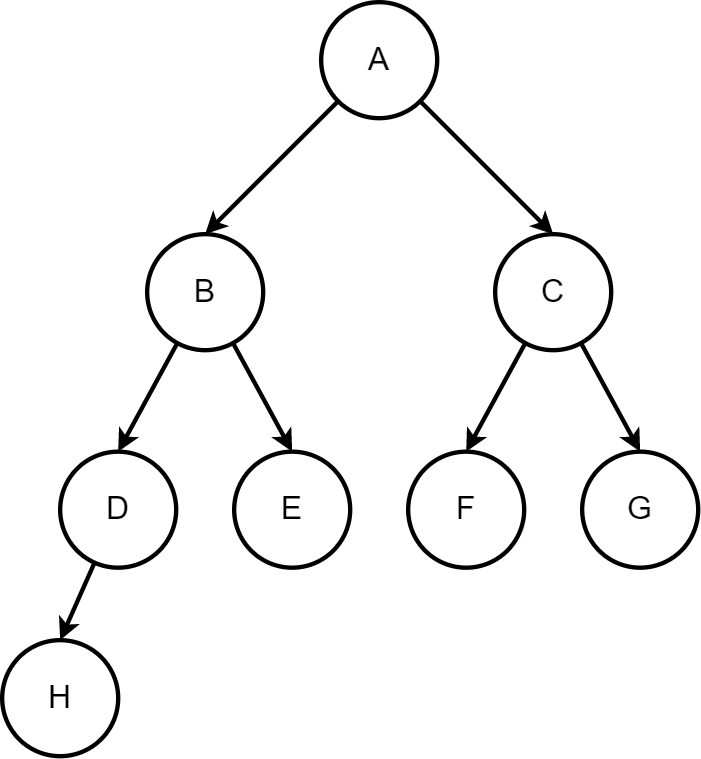
\includegraphics[height=0.6\textheight]{src/ett_1.png}
            \end{center}
        \end{itemize}
    \end{frame}

    \begin{frame}{樹壓平 Euler Tour Technique}
        \begin{center}
            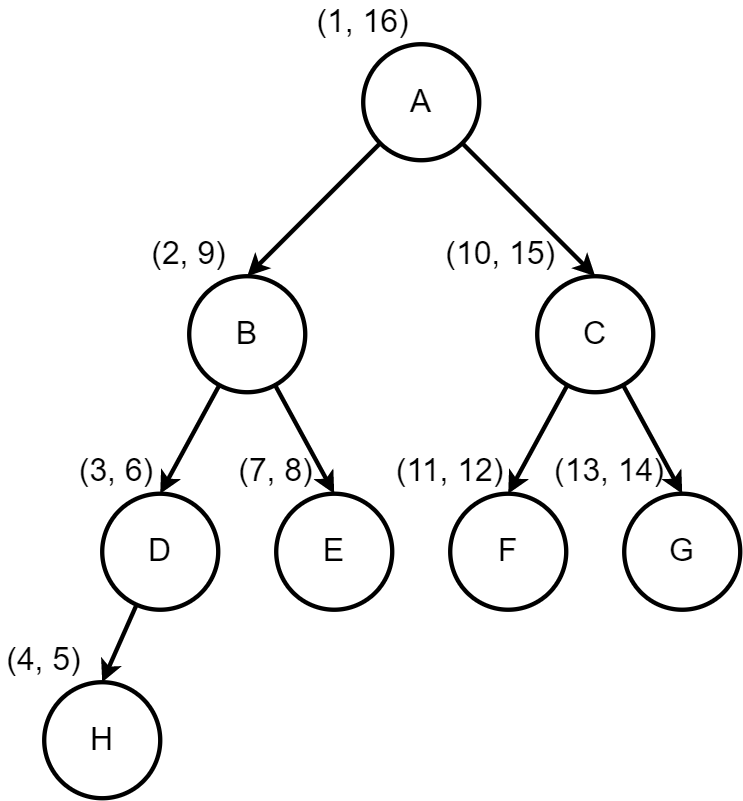
\includegraphics[height=0.8\textheight]{src/ett_2.png}
        \end{center}
    \end{frame}

    \begin{frame}{樹壓平 Euler Tour Technique}
        \begin{itemize}
            \item 如此一來我們就可以得到一個樹序列
        \end{itemize}

        \begin{center}
            \begin{tabular}{c|c|c|c|c|c|c|c|c|c|c|c|c|c|c|c|c}
                ett & 01 & 02 & 03 & 04 & 05 & 06 & 07 & 08 & 09 & 10 & 11 & 12 & 13 & 14 & 15 & 16\\
                \hline
                V & A & B & D & H & H & D & E & E & B & C & F & F & G & G & C & A
            \end{tabular}
        \end{center}

        \begin{itemize}
            \item<1-> 那這個樹序列可以做什麼事呢?
            \item<2-> 觀察一下序列中兩個同樣字母之間的字母
            \item<3-> 可以發現到,時間戳記位在某個點 $u$ 入點及出點之間的點,就是 $u$ 的子孫
            \item<4-> 所以我們可以利用樹序列來快速求得某個點 $v$ 是否為點 $u$ 的子孫
            \item<5-> 這個技巧經常用來處理一些樹上的操作,例如 LCA (共同最長子序列) 或是一些樹上的區間操作等等
            \item<5-> 參考程式:ett.cpp
        \end{itemize}
    \end{frame}

    \begin{frame}{樹壓平例題}
        \begin{block}{ABC 187E}
            有一 $n$ 個節點、$n-1$ 條邊的樹,第 $i$ 條邊連接 $a_i, b_i$,每個結點一開始都有一個值 $c_i$,$c_i$ 一開始都是 $0$\\
            共有 $q$ 次操作,對於第 $i$ 次操作輸入 $t_i, e_i, x_i$ 有兩種情況:
            \begin{enumerate}
                \item $t_i = 1$:對於所有 $a_{e_i}$ 能走到且不經過 $b_{e_i}$ 的點,將他們的 $c_i$ 全部加上 $x_i$
                \item $t_i = 2$:對於所有 $b_{e_i}$ 能走到且不經過 $a_{e_i}$ 的點,將他們的 $c_i$ 全部加上 $x_i$
            \end{enumerate}
            求做完所有操作之後,每個點的 $c_i$ 都是多少?$(n, q \le 2 \times 10^5)$
        \end{block}

        \begin{itemize}
            \item<1-> 先來解讀一下操作的意思:
            \item<2-> 假設 $dep(a_{e_i}) < dep(b_{e_i})$,那麼對於所有 $a_{e_i}$ 能走到且不經過 $b_{e_i}$ 的點就是除了 $b_{e_i}$ 的子孫的所有點,反之就是 $b_{e_i}$ 的子孫
            \item<3-> 所以我們需要做的事情就是將某個點的祖先或是子孫的 $c_i$ 全部加上 $x_i$
            \item<4-> 判斷子孫的部分剛剛講過了,要判斷點 $v$ 是否為點 $u$ 的祖先我們只需要判斷 $intime(v) > intime(u)$ 即可
        \end{itemize}
    \end{frame}
    
    \begin{frame}{樹壓平例題}
        \begin{itemize}
            \item<1-> 定義 $cnt[i]$ 是第 $i$ 個時間點走到的點的 $c_i$ 值
            \item<1-> 假設要操作的點是 $a, b$ 且 $dep(a) < dep(b)$
            \item<2-> 那麼當 $t_i = 1$ 時,就是將除了 $[intime[b], outtime[b]]$ 以外的時間都加上 $x_i$,也就是將 $[1, intime[b]), (outtime[b], n * 2]$ 都加上 $x_i$
            \item<2-> 反之,如果 $t_i = 2$,就是將 $[intime[b], outtime[b]]$ 都加上 $x_i$
            \item<2-> 至於 $dep(a) > dep(b)$ 就是相反
        \end{itemize}
    \end{frame}

    \begin{frame}{樹壓平例題}
        \begin{itemize}
            \item<1-> 如果一個一個加的話時間複雜度會是恐怖的 $\mathcal{O}(nq)$
            \item<2-> 我們可以將 cnt 畫成 $x-y$ 圖
            \begin{center}
                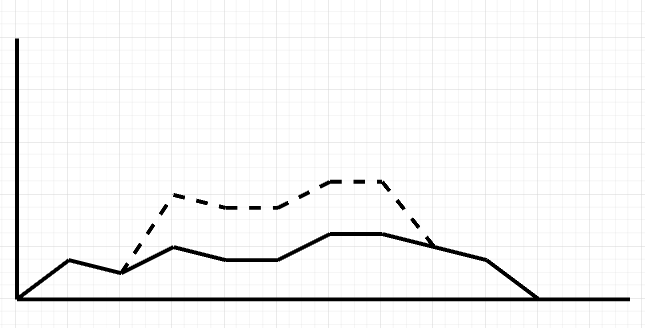
\includegraphics[height=0.6\textheight]{src/abc187e.png}
            \end{center}
        \end{itemize}
    \end{frame}

    \begin{frame}{樹壓平例題}
        \begin{itemize}
            \item<1-> 如果我們觀察斜率的話,可以發現到斜率只有在起點跟終點有變化而已
            \item<2-> 我們或許可以不維護 $c_i$,而是維護 $c_i - c_{i-1}$,也就是斜率
            \item<2-> 如此一來我們每次操作就只需要修改兩個點就可以了
            \item<3-> 最後要還原出 $c_i$ 的值,就只需要算出前綴和就可以了
            \item<3-> 這樣維護斜率而降低操作次數的數列就叫做\textbf{差分數列}
        \end{itemize}
    \end{frame}

    \begin{frame}{樹壓平例題}
        \begin{itemize}
            \item<1-> 結合以上兩點,我們就可以整理出 $dep(a) < dep(b)$ 時的操作方式:
            \item<2-> $t_i = 1$:cnt[1] += x, cnt[intime[b]] -= x, cnt[outtime[b] + 1] += x, cnt[n * 2 + 1] -= x
            \item<2-> $t_i = 2$:cnt[intime[b]] += x, cnt[outtime[b] + 1] += x
            \item<3-> 最後,如果要求出每個時間點確切的 $c_i$ 值,就只需要對 cnt 做前綴和就好了!
            \item<4-> 因為我們在做樹壓平的時候有紀錄每個時間點走到的點是哪一個,所以可以直接利用樹壓平所記錄的資訊將 $cnt$ 轉換成每個點的 $c_i$
            \item<4-> 時間複雜度:$\mathcal{O}(n + q)$
            \item<4-> 參考程式:ABC187E.cpp
        \end{itemize}
    \end{frame}



    \begin{frame}{BFS 廣度優先搜尋}
        \begin{itemize}
            \item 將 BFS 改成在圖論上也是同理
            \item 將枚舉點的步驟改成是枚舉相鄰的點即可
            \item 需要注意的是,DFS 因為是遞迴,所以呼叫了就會馬上執行,但 BFS 是用 queue,所以在 push 的時候必須同時更新該點已經走過\
            否則可能會產生一個點被多次 push 的情況發生,這會導致你的複雜度直接爆炸
            \item 參考程式:bfs\_1.cpp
        \end{itemize}
    \end{frame}

    \begin{frame}{BFS 例題}
        \begin{block}{CSES 1667 Message Route}
            Sam 的網路有 $n$ 台電腦還有 $m$ 條網路線,每條網路線連接電腦 $a_i, b_i$\\
            求從電腦 $1$ 傳輸資料到電腦 $n$ 的最短路徑,並將其構造出來 $(n \le 10^5, m \le 2 \times 10^5)$
        \end{block}

        \begin{itemize}
            \item<1-> 求出最短需要幾步之後,要怎麼構造出路徑呢
            \item<2-> 我們可以紀錄每一個點是從哪裡走過來的
            \item<3-> 全部走過之後,從終點往回走,並且把經過的點都記錄下來
            \item<3-> 就可以得到一組最短路徑了
            \item<3-> 參考程式:Message\_Route.cpp
        \end{itemize}
    \end{frame}

    \section{二分圖 Bipartite graph}

    \begin{frame}{什麼是二分圖}
        一張圖的節點分為兩個集合,且集合內部沒有邊的圖\\
        如果將點塗為黑色或白色 (0/1),那麼一個合法的二分圖中的每條邊必連接一黑點及一白點
    \end{frame}

    \begin{frame}{二分圖}
        \begin{block}{塗顏色問題}
            現在給你一張圖,你可以把每個節點塗成黑色或白色,但是每條邊相鄰的兩個點需要塗不同顏色\\
            求能不能成功塗色
        \end{block}

        \begin{itemize}
            \item<1-> 我們或許可以使用位元枚舉來枚舉每個點是不是 0 (黑色) 還是 1 (白色),但這樣要 $\mathcal{O}(2^n)$,顯然太慢了
            \item<2-> 我們可以先觀察到一個性質:
            \item<2-> 如果有一個點 $u$ 被塗成黑色,那麼所有跟 $u$ 相鄰的點 $v$ 就一定只能被塗成白色
            \item<3-> 那我們就可以從一個點開始塗,然後不斷的將與其相鄰的點塗成相反顏色就好
            \item<3-> 可以用 dfs / bfs 來實作
            \item<4-> 如果塗到一半發現有一個相鄰的點已經被塗過了,且該點的顏色跟目前點的顏色一樣,那就代表出現非法的情況了
        \end{itemize}
    \end{frame}

    \begin{frame}{二分圖例題}
        \begin{block}{CSES 1668 Building Teams}
            NHDK 有 $n$ 個人,其中有 $m$ 條朋友關係,Sam 希望將這 $n$ 個人分成兩組,且在同一組的人都沒有朋友關係\\
            求出一組分組方式
        \end{block}

        \begin{itemize}
            \item 基本上只需要將 dfs 過程中紀錄的塗色結果輸出出來就好了
            \item 參考程式:Building\_Teams.cpp
        \end{itemize}
    \end{frame}

    \begin{frame}{二分圖例題}
        \begin{block}{TPR17 pD New Year}
            TPR 國的總統想要將 TPR 國內的家庭分成兩組,並且另有姻親關係的兩個家庭會被分成不同的組別\\
            總統以為自己很聰明,所以他先自己分了一次,但其實他分出來的錯誤率很大,為了不要打擊他的自尊心,
            請問總統提出的方案需要更改幾個家庭的分組才能夠使其合法,若沒有辦法的話則輸出 -1
        \end{block}

        \begin{itemize}
            \item<2-> 可以觀察到一個性質
            \item<2-> 一個滿足二分圖的連通塊中,只有兩種分組方式
            \item<3-> 那我們就針對每個連通塊,看哪種分組方式跟總統的最接近,那就選那個方案就好
            \item<3-> 參考程式:TPR17\_PD.cpp
        \end{itemize}
    \end{frame}

    \begin{frame}{二分圖例題}
        \begin{block}{APCS 202111 P4 真假子圖 (ZJ g598)}
            NHDK 有 $n$ 個工作人員,工作人員被分成 $A, B$ 兩組,\
            並且一個人 $x$ 可能會跟另外一個人 $y$ 合作,稱為一組合作關係,且 $x, y$ 不會在同一組內\\
            Colten 原先有每組合作關係的名單,但是因為一些因素遺失了一部分,只剩下 $m$ 組合作關係,\
            所以他派出了 $p$ 個調查員來合作關係,每個調查員都會回傳 $k$ 組合作關係\\
            但是調查員回傳的資料可能不是正確的,也就是可能不會滿足兩個人不在同一組內,\
            請你求出有哪些調查員的資料是錯誤的,已知回傳錯誤資料的調查員不超過三位
        \end{block}

        \begin{itemize}
            \item<2-> 可以發現到,如果將一組合作關係的 $x_i, y_i$ 連成一條邊,那麼滿足兩人不在同一組內其實就是要滿足這張圖是一個二分圖
            \item<3-> 那麼我們其實可以一個一個加邊,如果發現加上這條邊之後會使得這張圖不是一個二分圖,那就代表這個調查員的資料是錯的
            \item<4-> 但以我們目前所學的東西,並沒有辦法在非 $\mathcal{O}(p \mid E\mid)$ 的時間做出來
        \end{itemize}
    \end{frame}

    \begin{frame}
        \begin{block}{APCS 202111 P4 真假子圖 (ZJ g598)}
            NHDK 有 $n$ 個工作人員,工作人員被分成 $A, B$ 兩組,\
            並且一個人 $x$ 可能會跟另外一個人 $y$ 合作,稱為一組合作關係,且 $x, y$ 不會在同一組內\\
            Colten 原先有每組合作關係的名單,但是因為一些因素遺失了一部分,只剩下 $m$ 組合作關係,\
            所以他派出了 $p$ 個調查員來合作關係,每個調查員都會回傳 $k$ 組合作關係\\
            但是調查員回傳的資料可能不是正確的,也就是可能不會滿足兩個人不在同一組內,\
            請你求出有哪些調查員的資料是錯誤的,已知回傳錯誤資料的調查員不超過三位
        \end{block}

        \begin{itemize}
            \item<1-> 但是我們可以觀察到一個性質
            \item<2-> 當加入了一條邊會使其變得不合法之後,不管後面再加了甚麼邊,都不會再變成合法的了
            \item<2-> 這其實就是某種單調性
            \item<3-> 想到單調性就會想到二分搜,所以我們可以對他二分搜找出提供錯誤資料且還沒被發現的調查員中編號最小的一個
        \end{itemize}
    \end{frame}

    \begin{frame}
        \begin{block}{APCS 202111 P4 真假子圖 (ZJ g598)}
            NHDK 有 $n$ 個工作人員,工作人員被分成 $A, B$ 兩組,\
            並且一個人 $x$ 可能會跟另外一個人 $y$ 合作,稱為一組合作關係,且 $x, y$ 不會在同一組內\\
            Colten 原先有每組合作關係的名單,但是因為一些因素遺失了一部分,只剩下 $m$ 組合作關係,\
            所以他派出了 $p$ 個調查員來合作關係,每個調查員都會回傳 $k$ 組合作關係\\
            但是調查員回傳的資料可能不是正確的,也就是可能不會滿足兩個人不在同一組內,\
            請你求出有哪些調查員的資料是錯誤的,已知回傳錯誤資料的調查員不超過三位
        \end{block}

        \begin{itemize}
            \item<1-> 我們可以寫一個 check(mid) 代表使用調查員 $1 \sim mid$ 的資料是否會是合法的
            \item<2-> 判斷合法一樣使用 DFS 就可以了
            \item<3-> 但我們要怎麼知道哪些邊是第 $1 \sim mid$ 的調查員回傳的呢?
            \item<4-> 我們可以將存圖的 vector<int> 改成 vector<pair<int, int>>,在 second 的地方存調查員的編號,在 DFS 時只走訪 second 是 $1 \sim mid$ 的邊就可以了
        \end{itemize}
    \end{frame}

    \begin{frame}
        \begin{block}{APCS 202111 P4 真假子圖 (ZJ g598)}
            NHDK 有 $n$ 個工作人員,工作人員被分成 $A, B$ 兩組,\
            並且一個人 $x$ 可能會跟另外一個人 $y$ 合作,稱為一組合作關係,且 $x, y$ 不會在同一組內\\
            Colten 原先有每組合作關係的名單,但是因為一些因素遺失了一部分,只剩下 $m$ 組合作關係,\
            所以他派出了 $p$ 個調查員來合作關係,每個調查員都會回傳 $k$ 組合作關係\\
            但是調查員回傳的資料可能不是正確的,也就是可能不會滿足兩個人不在同一組內,\
            請你求出有哪些調查員的資料是錯誤的,已知回傳錯誤資料的調查員不超過三位
        \end{block}

        \begin{itemize}
            \item<1-> 找到一個提供錯誤資訊的調查員之後,我們可以將他標計為非法,之後在做 DFS 時也忽略該調查員提供的資料即可
            \item<2-> 因為已知錯誤的調查員最多只有 3 個,所以我們只需要二分搜 3 次就可以得到答案了
            \item<3-> 時間複雜度 $\mathcal{O}(p\log \mid E \mid)$
            \item<3-> 據說這一場只有五個人滿級分
            \item<3-> 參考程式:g598.cpp
        \end{itemize}
    \end{frame}

    \section{拓撲排序}

    \begin{frame}{什麼是拓撲排序}
        \begin{itemize}
            \item<1-> 拓撲排序是用來解決圖上點的順序的方法
            \item<1-> 跟一般的排序無關
            \item<2-> 能夠做拓撲排序的圖必定是一張有向無環圖 (DAG)
            \item<2-> 換句話說,要驗證一張圖是否是有向無環圖就可以用拓撲排序來驗證
        \end{itemize}
    \end{frame}

    \begin{frame}
        \begin{block}{拓撲排序的例子}
            想像你今天是一位大學生,你需要修一些課,\
            但有些課需要先修完某些其他的課才能夠修,例如 $A$ 上完才可以上 $B$,$B$ 上完才可以上 $C$
        \end{block}

        \begin{itemize}
            \item<1-> 這種情況顯然就是 $A\rightarrow B \rightarrow C$ 嘛
            \item<2-> 那如果是 $A$ 上完才可以上 $B$,$B$ 上完才可以上 $C$,$C$ 上完才可以上 $A$ 呢?
            \item<3-> 我們就會發現它產生了矛盾,找不到一組拓撲排序
            \item<4-> 拓撲排序就是在解決這類型的問題
        \end{itemize}
    \end{frame}

    \begin{frame}{如何求拓撲排序}
        \begin{itemize}
            \item<1-> 拓撲排序主要有兩種求法
            \begin{enumerate}
                \item DFS
                \item Kahn 演算法
            \end{enumerate}
            \item<2-> 在找拓撲排序之前,我們需要先將關係圖建成一張圖
            \item<3-> 如果需要先修 $u$ 才能修 $v$ 的話,我們會建一張由 $u$ 連向 $v$ 的邊
        \end{itemize}
    \end{frame}

    \begin{frame}{DFS 求拓撲排序}
        \begin{itemize}
            \item<1-> 剛剛有說到,是一張有向無環圖就沒有辦法拓撲排序
            \item<1-> 所以我們的首要目的就是要找出這張圖有沒有環
            \item<2-> 假設我們在 dfs 的時候走到了一個點 $u$,與其相鄰的點 $v$ 中有任意一個存在於目前所走的路徑上,那就代表這張圖有環
            \item<2-> 那該如何得知一個點在目前所走的路徑上呢?
            \item<3-> 我們通常會開一個 vis[] 代表哪些點走過了,並且在走到一個點 $i$ 的時候就把 vis[i] 標為 1
            \item<4-> 我們可以擴充一下,如果點 $i$ 在目前走的路徑上,就標為 2,而退出該點的時候再標回 1 代表該點走過但並沒有位在目前的路徑上
            \item<5-> 如此一來,我們就能夠寫出一個能夠判斷一張圖有沒有環的 DFS 了
        \end{itemize}
    \end{frame}

    \begin{frame}{求是否有環的練習}
        \begin{block}{CSES 1669 Round Trip}
            TPR 國有 $n$ 座城市,其中有 $m$ 條道路\\
            請問是否有一個路徑起終點相同,且經過的城市數量 $> 1$,如果有則將其構造出來 $(n \le 10^5, m \le 2 \times 10^5)$
        \end{block}

        \begin{itemize}
            \item<1-> 這一題除了要找到是否有環,還要構造出一組環的解
            \item<2-> 我們可以利用一個 stack 來儲存目前路徑上的點
            \item<3-> 如果遇到環的起終點 u (vis[u] == 2),那我們就將這個 stack 裡面的點都取出來,直到取到 $u$ 為止,那我們就可以成功地將這個環裡面的點都取出來了
            \item<3-> 參考程式:Round\_Trip.cpp
        \end{itemize}
    \end{frame}

    \begin{frame}{DFS 求拓撲排序}
        \begin{block}{CSES 1679 Course Schedule}
            給一張有向圖,輸出一組拓撲排序
        \end{block}

        \begin{itemize}
            \item<1-> 知道怎麼判斷非法情況之後,就要來構造出一組解了
            \item<2-> 可以發現到,在 DFS 的過程中,第一個走出去的點,也就是第一個沒有其他點可以走的點,就會是最後可以走的點
            \item<3-> 以此類推,第二個走出去的點,就是倒數第二個可以走的點
            \item<4-> 所以我們只要紀錄在 DFS 的過程中,出點的順序,最後再將他反轉,就可以得到一個拓撲排序了
            \item<4-> 參考程式:Course\_Schedule\_dfs.cpp
        \end{itemize}
    \end{frame}

    \begin{frame}{Kahn 演算法}
        \begin{block}{CSES 1679 Course Schedule}
            給一張有向圖,輸出一組拓撲排序
        \end{block}
        
        \begin{itemize}
            \item<1-> 觀察一下選課的例子,一門課可以選需要滿足什麼條件?
            \item<2-> 不難發現到,當修一門課前需要先修的課都修完,我們就可以修該門課
            \item<3-> 該怎麼把這個性質轉成圖論呢?
            \item<3-> 把這個性質轉成圖論之後,我們就可以得到一個規則:當一個點 $u$ 的所有入邊所連接的點 $v$ 都走過之後,$u$ 就可以走
            \item<4-> 我們可以得到一個策略:先從入度為 0 的點開始,每走到一個點 $u$,就把 $u$ 的出邊能走到的點的 $v$ 入度都 $-1$,當 $deg^+(v)=0$ 時,那就代表 $v$ 可以走了,那我們就將他放進 queue 當中
            \item<5-> 這其實就是有限制條件的 BFS
            \item<5-> 參考程式:Course\_Schedule\_bfs.cpp
        \end{itemize}
    \end{frame}

    \begin{frame}{複雜度分析}
        \begin{itemize}
            \item 時間複雜度:$\mathcal{O}(V)$
            \item 空間複雜度:$\mathcal{O}(V+E)$
        \end{itemize}
    \end{frame}

    \begin{frame}{拓撲排序例題}
        \begin{block}{CF 510C Fox And Names}
            Foxyy 想要出版一篇論文,他聽說作者列表總是會按照字典序排列,但他發現事實不是這樣,\\
            給你作者的列表,請問你有沒有辦法將字母的順序重新排列,使得作者列表滿足按照字典序排列?
        \end{block}

        \begin{itemize}
            \item<2-> 以第一筆範測的第 2、3 個作者為例:shamir 與 adleman 在比較字典序時,會比 s、a 哪個比較小
            \item<3-> 由於在作者列表裡 shamir < adleman,所以我們就可以得知在新的字母排列中,s < a,那麼我們就可以連一條 $s \rightarrow a$ 的邊
            \item<4-> 最後,依照我們所連的邊去做拓撲排序,就可以得到我們的答案了
            \item<4-> 參考程式:510C.cpp
        \end{itemize}
    \end{frame}

    \begin{frame}{拓撲排序例題}
        \begin{block}{CF 1385E Directing Edges}
            有一張混和圖,請問所有的無向邊定向之後能否使這張圖能夠被拓撲排序?\\
            如果可以,請輸出 YES 以及所有邊的內容,否則請輸出 NO。$(n \le 2 \times 10^5)$
        \end{block}

        \begin{itemize}
            \item<2-> 可以發現到,一條無向邊的存在並不影響一張圖能否拓撲排序
            \item<3-> 因為一條邊所連接的兩點,一定有一個點是比較早走,一個是比較晚走的
            \item<4-> 所以我們只需要考慮包含有向邊的子圖
            \item<5-> 得出了拓撲排序的順序之後,再將無向邊定向為早走的點 $\rightarrow$ 晚走的點即可
            \item<5-> 參考程式:1385E.cpp
        \end{itemize}
    \end{frame}

    \begin{frame}{求最小字典序的拓撲排序}
        \begin{block}{ABC 223D Restricted Permutation}
            求出一組最小字典序的拓撲排序
        \end{block}

        \begin{itemize}
            \item<1-> 因為字典序是優先比較前面的元素,所以我們可以得到一個策略:優先走編號小的點
            \item<2-> 因為 queue 裡面的元素就是目前可以走的點,所以我們要執行這個策略就只需要在 queue 裡面挑最小的點走
            \item<3-> queue、取最小值,應該不難想到可以使用 priority\_queue
            \item<3-> 只需要將 queue 改成 priority\_queue 就可以達成求最小字典序了
            \item<3-> 參考程式:topo\_mindict.cpp
        \end{itemize}
    \end{frame}

    \section{DAG 上 DP}

    \begin{frame}{DAG 上 DP}
        \begin{itemize}
            \item 還記得早上的 DP 課嗎
            \item 如果今天把 DP 搬到了 DAG 上呢?
        \end{itemize}
    \end{frame}

    \begin{frame}{DAG 上 DP}
        \begin{block}{Atcoder DP Contest pG Longest Path}
            給一個 DAG 的有向圖,求一條最長的路徑
        \end{block}

        \begin{itemize}
            \item<2-> 先假設他是一條鍊,且所有邊的方向都是一樣的
            \item<3-> 那我們可以很簡單的求出一個轉移式:dp[i] = max(dp[i], dp[i - 1] + 1)
            \item<4-> 可以發現到,我們所做的事情就是在從以前走過的點做轉移
            \item<4-> 也就是說,我們需要先走過前面的點,才能夠走後面的點
        \end{itemize}
    \end{frame}

    \begin{frame}{DAG 上 DP}
        \begin{block}{Atcoder DP Contest pG Longest Path}
            給一個 DAG 的有向圖,求一條最長的路徑
        \end{block}

        \begin{itemize}
            \item<1-> 那搬到圖上呢?
            \item<2-> 可以發現到,"需要先走過前面的點,才能夠走後面的點" 這個條件,在圖上其實就是拓撲排序的條件
            \item<3-> 所以我們在做轉移的時候,只需要按照拓撲排序的順序走訪並轉移就可以了
            \item<4-> 假設我們目前在點 $u$,與其相臨的點為 $v$ 那我們就可以得到一個轉移式:dp[v] = max(dp[v], dp[u] + 1)
            \item<4-> 參考程式:ATCDP\_pG.cpp
        \end{itemize}
    \end{frame}

    \begin{frame}{DAG 上 DP}
        \begin{block}{ABC 188E Peddler}
            有 $n$ 座城市,$m$ 條\textbf{單向}道路,第 $i$ 條道路連接 $a_i, b_i$,\\
            有一個商人想要在這 $n$ 座城市間交易,已知第 $i$ 座城市的交易價為 $p_i$ (買價與賣價相同),\\
            請問在只買賣各一次的情況下,商人最多可以獲利多少元? $(n, m \le 2 \times 10^5)$
        \end{block}

        \begin{itemize}
            \item<1-> 我們一樣先把他看成是一條鍊來想
            \item<2-> 在第 $i$ 個點賣掉商品的最大獲利就是 p[i] - min(p[j]) (j < i)
            \item<3-> 最後的答案就會是 ans = max(p[i] - min(p[j])) (j < i)
            \item<4-> 設 dp[i] 為 i 以前的最小買入價格,就可以得到最後的轉移式 ans = max(p[i] - dp[i])
            \item<5-> 最後,套上拓撲排序就可以了
            \item<5-> 參考程式:ABC188E.cpp
        \end{itemize}
    \end{frame}

    \section{總結}

    \begin{frame}{總結}
        \begin{itemize}
            \item 可以發現到,很多圖論演算法都是基於 DFS、BFS 去做延伸與修改的
            \item 所以要精熟圖論,就要先精熟 DFS、BFS
            \item 如果覺得很抽象的話,可以適度的把走訪順序都印出來
            \item 希望大家能夠對圖論有一定的熟悉
        \end{itemize}
    \end{frame}
\end{document}